\section{Проект}
\subsection{Средства реализации}
Для реализации приложения был выбран язык программирования C++, т.к. он очень распространен, что упрощает последующую поддержку приложения. К тому же, программы, написанные на этом языке, могут быть скомпилированы для очень большого количества платформ.

Для упрощения переноса приложения на другие платформы, был использован кроссплатформенный инструментарий разработки ПО под названием Qt. Он так же включает в себя инструментарий, необходимый для разработки кроссплатформенных приложений с графическим интерфейсом пользователя. Выбор этого инструментария позволяет уменьшить усилия, требуемые для реализации новой и поддержки имеющейся функциональности.

Для того, чтобы приложение могло задействовать как можно больше доступных ресурсов современных ПК, было решено использовать фреймворк OpenCL. Это позволит приложению задействовать ресурсы всех процессоров в многопроцессорных системах, а так же ресурсы современных видеокарт.
Для взаимодействия с OpenCL используется экспериментальный биндинг для языка C++~\cite{opencl_bindings}, который предоставляет ООП-интерфейс для доступа к OpenCL.

\section{Модули и алгоритмы}
Составляющими элементами системы являются библиотека covc и набор приложений:
\begin{itemize}
\item oclc
\item qcovc
\item ocl\_volume\_render
\end{itemize}


\subsection{Библиотека covc}
Библиотека covc содержит реализацию алгоритма раскраски вокселей методом множества гипотез.

\subsubsection{Программный интерфейс библиотеки}
Программный интерфейс библиотеки состоит из следующих функций:
\begin{itemize}
\item \textit{add\_image} -- добавление нового изображения
\item \textit{build\_voxel\_model} -- запуск алгоритма
\item \textit{get\_voxel\_model} -- получение результирующей вокселной модели
\item \textit{prepare} -- инициализация библиотеки
\item \textit{set\_camera\_calibration\_matrix} -- ввод матрицы внутренней калибровки камеры
\item \textit{set\_number\_of\_images} -- ввод количества изображений
\item \textit{set\_resulting\_voxel\_cube\_dimensions} -- ввод размерностей результирующей вокселной модели
\end{itemize}

\subsection{Алгоритм раскраски вокселей}
Все операции в процессе реконструкции производятся над вокселами, которые уникальны для трехмерной модели объекта, а не над пикселями, которых несколько для одного воксела. Поэтому не нужно специально вычислять точки соответствия и по ним вычислять карту глубины.

В реализованном алгоритме четыре этапа:
\begin{enumerate}
\item Вычисление объемлющего трехмерного куба объекта
\item Инициализация вокселей, назначение каждому вокселю гипотез
\item Первоначальная отбраковка ложных гипотез
\item Дальнейшая проверка гипотез на соответствие по всем изображениям и  удаление ложных гипотез
\end{enumerate}

\subsubsection{Вычисление объемлющего трехмерного куба объекта}
В начале работы программы можно ограничить пространство, в котором располагается реконструируемый объект. Для этого пользователь на изображениях выделяет рамкой объект. Затем, используя калибровочные данные, вычисляется объемлющий объект объем (bounding volume). Для его расчета на каждом отмеченном рамкой изображении считается двумерный центр этой рамки. Если рамка не задана, то в используется двумерный центр изображения. По всем полученным двумерным центрам и матрицам внешней калибровки считается трехмерный центр всех рамок, отмеченных пользователем, и изображений. Впоследствии этот центр будет центром полученного объемлющего куба.

Трехмерные координаты камеры $[x;y;z]^T$ можно найти так:

\begin{center}
	$[x;y;z;w]^T = C^{-1}*[0;0;0;1]^T$ , где
\end{center}
$C$ - матрица внешней калибровки изображения, полученного с этой камеры.

Каждое изображение относительно своей камеры находится на расстоянии~1. Считаем трехмерные координаты $[X_{3D};Y_{3D};Z_{3D}]^T$ углов отмеченных рамок и изображений следующим образом:

\begin{center}
	$K^{-1}*[x;y;1]^T = [X;Y;Z]^T$ \\
	$[X_{3D};Y_{3D};Z_{3D}]^T = C^{-1}*[X;Y;Z]^T$ , где
\end{center}
$C$ - матрица внешней калибровки изображения;\\
$K$ - матрица внутренней калибровки камеры;
$[x;y;1]$ - координаты в пикселях угла выделенной рамки или изображения.

На рисунке ниже $OD = 1$; треугольник ${OAD}$ подобен треугольнику ${OBC}$. Требуется вычислить координаты точки $B$, если известны трехмерные координаты $A$, $O$, $C$:

\begin{center}
	$\frac{OB}{OA} = \frac{OC}{OD} = \frac{OC}{1} \Rightarrow OB = OA*OC$ \\
	$B = O + AO*OC$
\end{center}

\begin{figure}[h]
\center
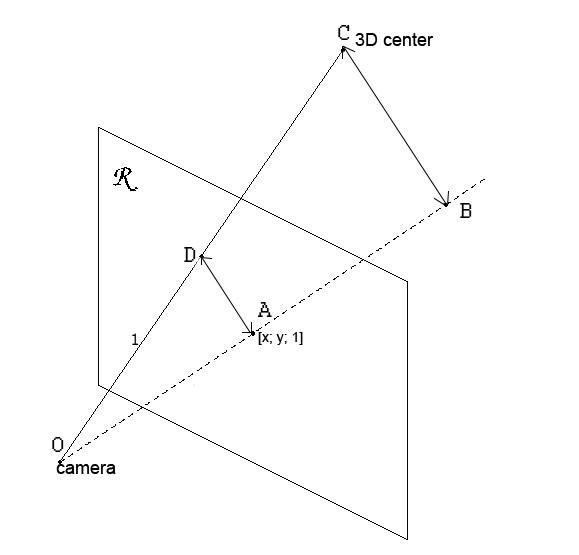
\includegraphics[scale=0.5]{3dcenter}
\caption{Вычисление трехмерных координат точек изображения}
\end{figure}

Таким образом, вычисляем трехмерные координаты всех углов отмеченных пользователем рамок. Далее можем вычислить трехмерную высоту и ширину выделенной рамки для каждого изображения. Считаем максимум среди этих расстояний. Полученное значение будем считать за сторону трехмерного куба, объемлющего объект.

\subsubsection{Инициализация вокселей, назначение каждому вокселю гипотез}
На следующем этапе для каждого изображения составляется матрица проекции:

\begin{center}
	$P = K*I*C$, где
\end{center}
$K$ - матрица внутренней калибровки камеры
$I$ - единичная матрица
$C$ - матрица внешней калибровки изображения.

Проекция воксела на изображение (координаты $x$ и $y$ в пикселях) получается умножением слева матрицы проекции данного изображения на трехмерный центр воксела:

\begin{center}
	$[x;y;z]^T = P*[X_{3D};Y_{3D};Z_{3D};1]^T$ \\
	$x = x/z$ \\
	$y = y/z$
\end{center}

Обходя все вокселы, для каждого воксела составляем гипотезы. Каждая гипотеза – это цвет проекции воксела на изображение в цветовом пространстве RGB. Для увеличения надежности алгоритма каждая компонента цвета гипотезы делится на сумму всех компонент (red + green + blue) этой гипотезы. Итого, для каждого воксела должно быть столько гипотез, сколько изображений во входной последовательности. Но если проекция воксела на изображение -- точка с пиксельными координатами $[x;y]$ -- выходит либо за границы изображения, либо за пределы выделенной пользователем рамки, соответствующая гипотеза считается ложной.

Сначала все вокселы видимые. Если все гипотезы для какого-либо воксела оказались ложными, этот воксел считается невидимым.

\subsubsection{Первоначальная отбраковка ложных гипотез}
Проходя последовательно по всем вокселам, для каждой гипотезы текущего воксела сравниваем ее со всеми остальными гипотезами для этого воксела. Гипотеза(1) считается верной, если найдется другая гипотеза(2) данного воксела, такая, что расстояние между этими гипотезами в цветовом пространстве RGB меньше заданного порога $T$:

\begin{center}
	$\lvert {red(0)} - {red(1)}\rvert + \lvert {green(0)} - {green(1)}\rvert + \lvert {blue(0)} - {blue(1)}\rvert < T$
\end{center}

Получим, что гипотеза ложная только в том случае, когда она не соответствует ни одной другой гипотезе для данного воксела. Так же как и ранее воксел считается невидимым, если все связанные с ним гипотезы ложны.

Далее считается, сколько осталось верных гипотез и изменяется порог $T$:

\begin{center}
	$T_{new} = T/{dim_x*dim_y*dim_z*N}$, где
\end{center}
$T_{new}$ - новое значение порога;\\
$dim_x, dim_y, dim_z$ - размерности результирующей модели по $x,y,z$ соответственно;\\
$N$ - количество изображений во входной последовательности.

Такое изменение порога позволяет более точно в дальнейшем определять ложные гипотезы.

\subsubsection{Дальнейшая проверка гипотез}

Алгоритм построен так, что он учитывает с какой стороны нужно рассматривать объемлющий куб для каждого изображения. Это сделано для того, чтобы правильно устанавливать видимость вокселей с каждого изображения. 

Чтобы найти порядок обхода вокселей для данного изображения, вычисляем расстояния в трехмерных координатах между камерой и всеми восемью углами объемлющего куба. Ближайший угол определяет порядок обхода вокселей: этот угол нужно обойти раньше остальных. 

В соответствующем порядке обходим куб и отбраковываем гипотезы как ранее:   
гипотеза ложная только в том случае, когда она не соответствует ни одной другой гипотезе для данного воксела, то есть:

\begin{center}
	$\lvert {red(i)} - {red(j)}\rvert + \lvert {green(i)} - {green(j)}\rvert + \lvert {blue(i)} - {blue(j)}\rvert > T_{new}$
\end{center}
при фиксированном $i$ для всех $i \neq j$.

Кроме того, для каждого изображения заводятся буфера – матрицы той же размерности, что и сами изображения на которых будут отмечаться видимые вокселы. Первоначально буфера пусты. Рассматривая каждую гипотезу проверяем, занят ли буфер на ее месте. Для этого вычисляем, какому вокселу соответствует эта гипотеза, Проецируем воксел на текущее изображение. Если буфер не занят, то заполняем его в тех  позициях, куда проецируется весь воксел (это может быть несколько пикселей). Если же буфер уже занят, то данный воксел не видим на этом изображении, и его гипотезу можно не рассматривать.    

Так обходятся все изображения в нужном порядке до тех пор, пока хоть одна гипотеза признается ложной. 

В итоге получаем вокселную модель реконструируемого объекта.

\newpage
\subsection{Реализация алгоритма}
Схематически алгоритм изображен на диаграмме ниже.
\begin{figure}[h]
\center
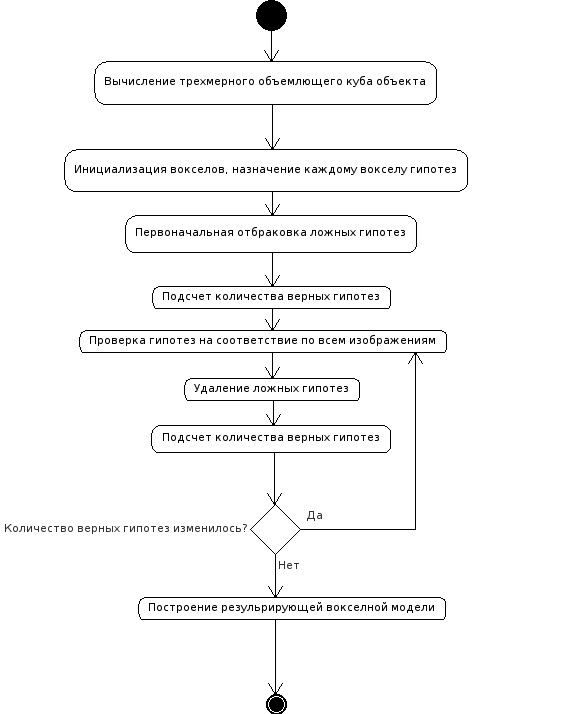
\includegraphics[scale=0.7]{qcovcactivitydiagram}
\caption{Диаграмма активности}
\end{figure}

На этапах <<Инициализация вокселей, назначение каждому вокселу гипотез>>, <<Первоначальная отбраковка ложных гипотез>>, <<Подсчет количества верных гипотез>> и <<Удаление ложных гипотез>> было применено распараллеливание вычислений.

\subsection{Приложение oclc}
Данное приложение является оберткой над компилятором OpenCL C. Оно позволяет проверить на корректность программы, написанные на языке OpenCL C и получить описание допущенных ошибок.

\subsection{Приложение qcovc}
Данное приложение позволяет пользователю, при помощи графического интерфейса, работать с библиотекой.

\subsubsection{Классы приложения}
\begin{itemize}
\item \textit{MainWindow} -- главное окно приложения
\item \textit{ImageInfo} -- информация об изображении
\item \textit{ImagePreview} -- виджет предпросмотра изображений
\item \textit{ImageScene} -- сцена для отображения изображения
\end{itemize}

\subsubsection{Класс MainWindow}
Методы класса:
\begin{itemize}
\item \textit{add\_image} -- добавление нового изображения
\item \textit{load\_metafile} -- загрузка метафайла
\item \textit{save\_metafile} -- сохранение метафайла
\end{itemize}

\subsubsection{Класс ImagePreview}
Методы класса:
\begin{itemize}
\item \textit{add\_image} -- добавление нового изображения в блок предпросмотра
\item \textit{clear} -- очистка блока предпросмотра
\end{itemize}

\subsubsection{Класс ImageScene}
Методы класса:
\begin{itemize}
\item \textit{rectangle\_changed} -- изменяет параметры объемлющего прямоугольника для изображения
\item \textit{set\_rectangle} -- устанавливает объемлющий прямоугольник для отображения
\item \textit{set\_image} -- устанавливает изображение для отображения
\end{itemize}

\subsubsection{Диаграмма классов}
\begin{figure}[h]
\center
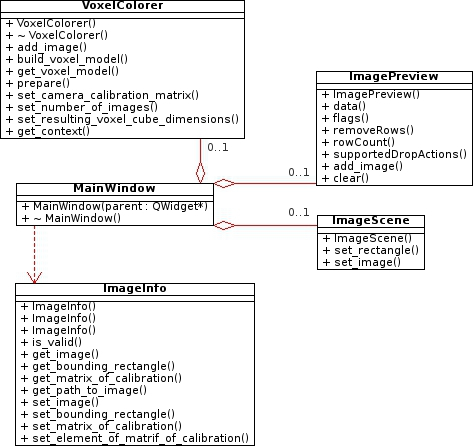
\includegraphics[scale=0.7]{qcovcclassdiagram}
\caption{Диаграмма классов приложения qcovc}
\end{figure}

\subsubsection{Проект интерфейса}
Из меню графического интерфейса пользователя должно быть доступно сохранение и загрузка метафайла, добавление нового изображения, запуск на выполнение алгоритма получения объемной модели объекта. Основное окно должно быть разделено на три части: слева должны находиться блок просмотра миниатюр изображений и блок ввода матрицы внешней калибровки камеры для выбранного изображения. Остальную часть окна должен занимать блок, в который выводится текущее выбранное изображение. Так же в этом блоке должно быть доступно выделение объемлющего прямоугольника.
\begin{figure}[h]
\center
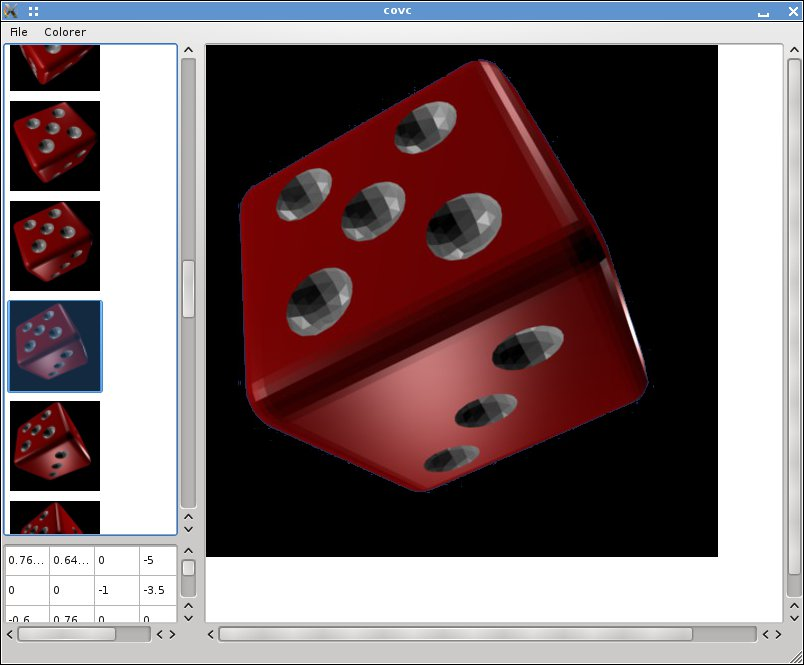
\includegraphics[scale=0.5]{gui}
\caption{Проект интерфейса}
\end{figure}

\newpage
\subsection{Приложение ocl\_volume\_render}
Данное приложение является модифицированной версией программы oclVolumeRender из комплекта NVIDIA GPU Computing SDK~\cite{nvidia_gpu_sdk} и позволяет пользователю просматривать полученную воксельную модель.


